% !TeX root = ../main.tex

\section{Introduzione}
In questo capitolo vengono inizialmente descritte le motivazioni che hanno spinto l'azienda Maggioli S.p.A.\footnote{\href{https://www.maggioli.com/en-us}{https://www.maggioli.com/en-us}} a dedicare risorse per la ricerca e la sperimentazione nei campi delle applicazioni multipiattaforma e delle tecniche DevOps in ambito mobile.
Successivamente sono indicati i requisiti del caso di studio industriale individuato, 
il quale può essere suddiviso in due macroaree:

\begin{itemize}
    \item definizione del processo di sviluppo per applicazioni multipiattaforma tramite l'adozione della cultura DevOps,
    
    \item sviluppo di un'applicazione mobile multipiattaforma utilizzando il processo di sviluppo definito.
\end{itemize}

\section{Contesto aziendale}
Tra i core business dell'azienda Maggioli S.p.A. è rimasto centrale il ruolo dell'editoria,
ma col trascorrere degli anni e il mutare delle esigenze dei clienti, 
i quali sono principalmente pubblica amministrazione (PA) e professionisti privati, 
come avvocati, 
architetti, 
commercialisti ed ingegneri edili, 
si è verificata una transizione verso il mondo digitale.

I servizi digitali erogati per la consultazione delle pubblicazioni hanno superato considerevolmente il formato cartaceo,
il quale rimane comunque un metodo secondario di consultazione disponibile seppur in forma molto ridotta. 
Per l'editoria digitale esiste in Maggioli una business unit dedicata, 
chiamata \textit{Digital Media}, 
il cui ruolo principale consiste nella realizzazione e manutenzione dei siti Web Maggioli dedicati alla ricerca e visualizzazione delle pubblicazioni digitali. 
I seguenti sono soltanto alcuni dei siti gestiti dal team \textit{Digital Media}: 
Biblioteca Digitale\footnote{\href{https://bibliotecadigitale.maggioli.it/}{https://bibliotecadigitale.maggioli.it/}}, 
Appalti \& Contratti\footnote{\href{https://www.appaltiecontratti.it/}{https://www.appaltiecontratti.it/}} e Periodici\footnote{\href{https://www.periodicimaggioli.it/}{https://www.periodicimaggioli.it/}}. 
La necessità principale è dunque quella di fare innovazione tramite lo sviluppo di un'applicazione mobile in modo da fornire ai clienti Maggioli un nuovo metodo di accesso alle pubblicazioni che sia più accessibile e comodo.

\begin{figure}[H]
    \centering
    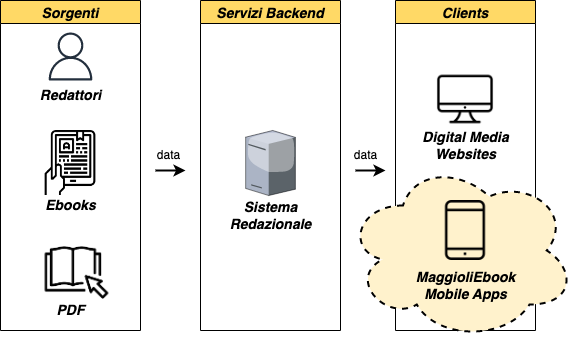
\includegraphics[width=0.75\textwidth]{img/contesto-aziendale.png}
    \caption{Schema del contesto aziendale in cui è collocato il caso di studio}
    \label{contesto-aziendale-fig}
\end{figure}

Le motivazioni che stanno alla base della scelta della cultura DevOps e delle applicazioni multipiattaforma per lo sviluppo di questo caso di studio sono comuni a qualsiasi tipologia di azienda: 
come descritto nei capitoli \ref{ch:devops} e \ref{ch:app-multiplatform} è possibile ottimizzare il processo di sviluppo diminuendo le risorse impiegate e quindi i costi ma allo stesso tempo aumentando la qualità del software e la frequenza di rilascio,
i quali comportano una maggiore soddisfazione sia da parte dell'utente finale che da parte dell'azienda.

\section{Definizione processo di sviluppo}
Considerando l'intero contesto aziendale esistono degli standard, 
consolidati con l'esperienza maturata nello sviluppo software, 
che devono essere adottati sia per quanto riguarda il processo di sviluppo che la scelta degli strumenti necessari. 
L'obiettivo è riuscire a definire un modello di processo fortemente basato sugli standard aziendali ma adattato alle esigenze dello sviluppo di applicazioni mobile multipiattaforma e che possa essere introdotto nei team che si occupano di applicazioni mobile. 
I principali standard aziendali riguardanti gli strumenti e le tecnologie che devono essere adottati sono:

\begin{itemize}
    \item \textbf{GitLab}\footnote{\href{https://about.gitlab.com/}{https://about.gitlab.com/}} (\textit{DVCS/CI Server}) - Le funzionalità necessarie al versionamento del codice, alla collaborazione/pianificazione e all'automazione (Sezione \ref{devops-tools-sec}) sono tutte soddisfatte dalla piattaforma cloud GitLab con la quale è presente una sottoscrizione di piano di licenza aziendale.
    
    \item \textbf{SonarQube}\footnote{\href{https://www.sonarqube.org/}{https://www.sonarqube.org/}} (\textit{Vulnerability Management System}) - Questo servizio self-hosted è reso disponibile a tutti i team aziendali e permette di soddisfare gran parte dei task di Continuous Inspection. Grazie a SonarQube è possibile effettuare l'analisi statica del codice, validare il rispetto di determinate policy aziendali e visualizzare dashboard sullo stato delle scansioni.
    
    \item \textbf{Renovate}\footnote{\href{https://docs.renovatebot.com/}{https://docs.renovatebot.com/}} (\textit{Dependency Management}) - Strumento utilizzato per automatizzare la gestione delle dipendenze dei progetti. 
\end{itemize}

La pipeline standard a livello aziendale, 
base di partenza per la definizione della pipeline per applicazioni mobile multipiattaforma, 
rispetta a pieno tutte le considerazioni fatte nel capitolo \ref{ch:devops} per tutte le tecniche d'automazione indicate (fig. \ref{ci-inspection-pipeline}). 
Tramite l'adattamento delle fasi di integration, delivery e inspection di questa pipeline con le necessità dello sviluppo mobile indicate nei capitoli \ref{ch:sdlc} e \ref{ch:app-multiplatform} si ottengono i seguenti requisiti e dunque la pipeline obiettivo da realizzare.

\subsection{Requisiti}
\begin{itemize}
    \item \textbf{R1} - Continuous Integration
    \begin{itemize}
        \item \textbf{R1.1} - Stage di compilazione, testing e packaging con i relativi sotto-task per entrambe le piattaforme Android e iOS.
        
        \item \textbf{R1.2} - L'output dell'ultimo stage deve essere un pacchetto contenente l'applicazione da passare come artefatto alla fase successiva di delivery.
        
        \item \textbf{R1.3} - Utilizzo del sistema aziendale di gestione automatica delle dipendenze Renovate.
    \end{itemize}
    
    \item \textbf{R2} - Continuous Delivery
    \begin{itemize}
        \item \textbf{R2.1} - Stage di stabilizzazione suddivisi tra \textit{Alpha} e \textit{Beta} per il testing interno ed esterno tramite gli appositi servizi forniti da Google e Apple: Google Play Console per l'applicazione Android e Testflight per l'applicazione iOS.
        
        \item \textbf{R2.2} - L'applicazione soggetta a stabilizzazione è data in input dalla fase precedente di integrazione.
        
        \item \textbf{R2.3} - Stage di pubblicazione sui relativi marketplace Google Play Store o App Store. L'applicazione soggetta a pubblicazione deriva dalla terminazione con successo della fase di stabilizzazione e si trova già sui portali utilizzati.
    \end{itemize}
    
    \item \textbf{R3} - Continuous Inspection
    \begin{itemize}
        \item \textbf{R3.1} - Stage di analisi statica e analisi delle dipendenze per entrambe le piattaforme.
        
        \item \textbf{R3.2} - Utilizzo del sistema aziendale di gestione delle vulnerabilità centralizzato SonarQube.
    \end{itemize}
    
    \item \textbf{R4} - Tutto il sistema di automazione deve poter essere utilizzato da altri team di sviluppo all'interno dell'azienda.
\end{itemize}

\begin{figure}[H]
    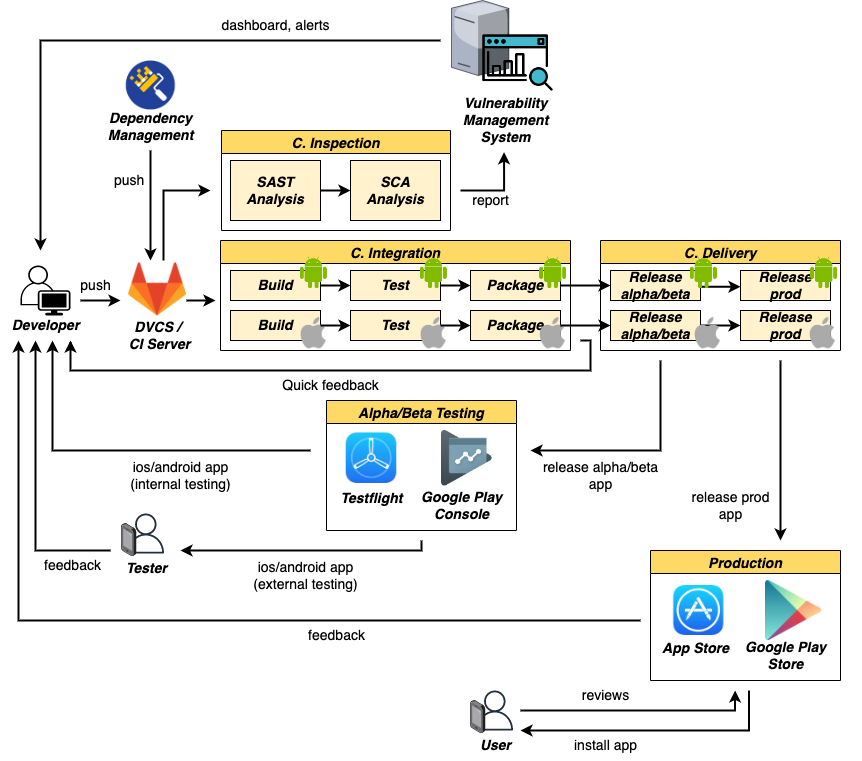
\includegraphics[width=1\textwidth]{img/full-cicd.png}
    \caption{Schema globale del processo di sviluppo automatizzato che si intende realizzare}
    \label{full-cicd}
\end{figure}

\section{Definizione applicazione}
Dato il contesto aziendale dell'editoria digitale in cui si colloca il caso di studio,
è possibile catalogare l'applicazione mobile da sviluppare come \textit{E-Reader}. 
Un e-book reader, 
chiamato anche e-book device o e-reader, 
è un dispositivo elettronico mobile progettato principalmente per la lettura di e-book e periodici digitali. 
Ogni dispositivo in grado di mostrare del testo su uno schermo potrebbe essere considerato un e-reader, 
ma i dispositivi progettati appositamente per questo compito hanno caratteristiche e funzionalità specifiche come l'ottimizzazione della portabilità, 
la leggibilità e la durata della batteria~\cite{shoba2014vocabulary}.

Per poter avere un valore aggiunto rispetto alle funzionalità già fornite dai siti Web sviluppati dal team \textit{Digital Media},
l'applicazione ``MaggioliEbook'' deve comportarsi come un vero e proprio e-reader, 
integrandosi ai servizi backend Maggioli per l'editoria digitale già esistenti. 
Data la complessità del dominio da modellare sono stati svolti degli incontri con figure interne esperte di dominio appartenenti ai team \textit{Ricerca e Sviluppo} e \textit{Digital Media}, 
al fine di definire (\textit{i}) terminologia, 
(\textit{ii}) casi d'uso e (\textit{iii}) requisiti.

\subsection{Terminologia e casi d'uso}
E' necessario che il team di sviluppo, 
composto da figure tecniche, 
e i committenti, 
i quali sono invece esperti interni di dominio, 
utilizzino lo stesso linguaggio per far si che le successive fasi del processo siano efficaci ed efficienti. 

Il concetto di \textit{Ubiquitous Language} definisce un vocabolario condiviso da entrambe le parti per la discussione del software~\cite{evans_domain-driven_2004} ed è stato adottato per la realizzazione del seguente glossario, 
il quale racchiude tutti i principali termini utilizzati negli incontri tra team di sviluppo ed esperti di dominio, 
suddivisi in \textit{entità} e \textit{casi d'uso}:

\subsubsection*{Entità}
\begin{table}[H]
\centering
    \begin{tabular}{|c|c|}
         \hline
         \textbf{Termine} & \textbf{Descrizione}\\
         \hline
         \textit{Reader} & \specialcell{Lettore di documenti in grado di visualizzarli ed \\interagire con essi.}\\
         \hline
         \textit{Documento} & Contenuto digitale pubblicato da Maggioli Editore.\\
         \hline
         \textit{Documento Statico} & Documento con una certa struttura definita (PDF).\\
         \hline
         \textit{Documento Fluido} & \specialcell{Documento senza struttura in grado di adattarsi al dispositivo\\ in cui viene aperto (EPUB).}\\
         \hline
         \textit{Libro} & \specialcell{Tipologia principale di documento fluido fruibile\\ tramite l'applicazione MaggioliEbook.}\\
         \hline
         \textit{Rivista} & \specialcell{Tipologia principale di documento statico fruibile\\ tramite l'applicazione MaggioliEbook.}\\
         \hline
         \textit{Bookmark} & Identifica una specifica pagina di un libro o di una rivista.\\
         \hline
         \textit{Progression} & \specialcell{Progresso di lettura di un libro o di una rivista,\\ calcolato in percentuale \\(numero di pagine lette sul totale del documento).}\\
         \hline
         \textit{Highlight} & \specialcell{Annotazione per una certa porzione testuale di \\documento. Può essere una evidenziazione, sottolineatura \\o annotazione testuale.}\\
         \hline
         \textit{Favorite} &  Documento preferito dall'utente.\\
         \hline
         \textit{User} & Utente con uno o più abbonamenti attivi.\\
         \hline
          \textit{Token} & \specialcell{Autentica e autorizza l'utente ad accedere ai vari documenti\\ per i quali esiste un abbonamento attivo.}\\
         \hline
    \end{tabular}
    \caption{Glossario dei termini (Entità)}
\end{table}

\newpage
\subsubsection*{Casi d'uso}
\begin{table}[H]
\centering
    \begin{tabular}{|c|c|}
         \hline
         \textbf{Termine} & \textbf{Descrizione}\\
         \hline
         \textit{Apertura Documento} & \specialcell{Richiesta di apertura in lettura di uno specifico\\ documento.}\\
         \hline
         \textit{Chiusura Documento} & Richiesta di chiusura del documento aperto in lettura.\\
         \hline
         \textit{Ricerca Documento} & Richiesta di ricerca documento tramite query testuale.\\
         \hline
         \specialcell{\textit{Lettura Metadati}\\\textit{Documento}} & Richiesta di lettura metadati documento.\\
         \hline
         \textit{Creazione Highlight} & Richiesta di creazione annotazioni.\\
         \hline
         \textit{Lettura Highlight} & Richiesta di lettura annotazioni.\\
         \hline
         \textit{Eliminazione Highlight} & Richiesta di eliminazione annotazioni.\\
         \hline
         \textit{Creazione Bookmark} & Richiesta di creazione segnalibri.\\
         \hline
         \textit{Lettura Bookmark} & Richiesta di lettura segnalibri.\\
         \hline
         \textit{Eliminazione Bookmark} & Richiesta di eliminazione segnalibri.\\
         \hline
         \textit{Creazione Progression} & \specialcell{Richiesta di salvataggio dell'\\avanzamento di lettura di un documento.}\\
         \hline
         \textit{Lettura Progression} &  \specialcell{Richiesta di lettura dell'\\avanzamento di lettura di un documento.}\\
         \hline
         \textit{Eliminazione Progression} &  \specialcell{Richiesta di eliminazione dell'\\avanzamento di lettura di un documento.}\\
         \hline
         \textit{Creazione Favorite} &  Richiesta di creazione preferiti.\\
         \hline
         \textit{Lettura Favorite} & Richiesta di lettura preferiti.\\
         \hline
         \textit{Eliminazione Favorite} & Richiesta di eliminazione preferiti.\\
         \hline
         \specialcell{\textit{Conversione}\\\textit{PDF2EPUB}} & \specialcell{Richiesta di conversione di un documento statico in\\ documento fluido (dal formato PDF al formato EPUB).}\\
         \hline
         \specialcell{\textit{Download Contenuto}\\\textit{Documenti}} & Scaricamento del contenuto dei documenti.\\
         \hline
         \specialcell{\textit{Download Copertina}\\\textit{Documenti}} & \specialcell{Scaricamento della immagine di copertina dei \\documenti.}\\
         \hline
         \textit{Login User} & Richiesta di login dell'utente (lettura token).\\
         \hline
         \textit{Logout User} & Richiesta di logout dell'utente (eliminazione token).\\
         \hline
         \specialcell{\textit{Controllo Login}\\\textit{User}} & \specialcell{Controllo di autenticazione dell'utente\\ già avvenuta (esistenza token).}\\
         \hline
         \specialcell{\textit{Lettura Account Utente}} & Richiesta informazioni utente (dati anagrafici e mail).\\
         \hline         
    \end{tabular}
    \caption{Glossario dei termini (Casi d'uso)}
\end{table}
\newpage

\begin{figure}[H]
\centering
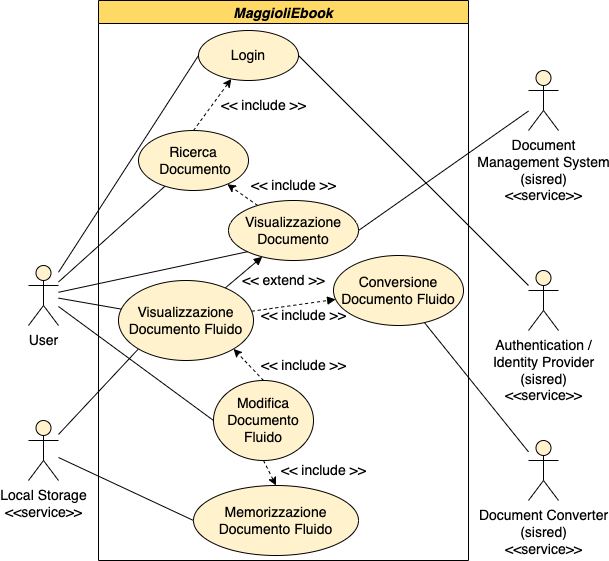
\includegraphics[width=1\textwidth]{img/casi-uso-uml.png}
\caption{UML - Diagramma dei casi d'uso: funzioni/servizi offerti dalla applicazione MaggioliEbook}
\end{figure}

\begin{figure}[H]
\centering
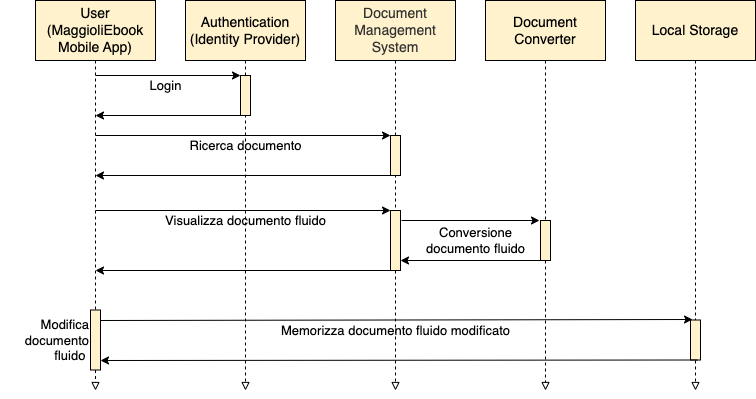
\includegraphics[width=1\textwidth]{img/caso-uso-sequenza-uml.png}
\caption{UML - Diagramma di sequenza: scenario di modifica di un nuovo documento "fluido"}
\end{figure}

\subsection{Requisiti}
\begin{itemize}
    \item \textbf{R1} - Visualizzazione documenti.
    \begin{itemize}
        \item \textbf{R1.1} - In modo fluido, mostrando il contenuto adattato al dispositivo in cui viene mostrato.
        
        \item \textbf{R1.2} - In modo statico, mostrando il contenuto con uno specifico layout indipendente dal dispositivo in cui viene mostrato.
    \end{itemize}
    
    \item \textbf{R2} - Modifica documenti fluidi (lato utente).
    \begin{itemize}
        \item \textbf{R2.1} - Aggiunta segnalibri, commenti, sottolineature, evidenziazioni, al contenuto fluido.
        
        \item \textbf{R2.2} - Memorizzazione segnalibri, commenti, sottolineature, evidenziazioni apportate al contenuto fluido.
    \end{itemize}
    
    \item \textbf{R3} - Gestione utente.
    \begin{itemize}
        \item \textbf{R3.1} - Login (autenticazione) utente.
        
        \item \textbf{R3.2} - Visualizzazione documenti a cui l'utente è abbonato.
    \end{itemize}
    
    \item \textbf{R4} - Ricerca documenti.
    
    \item \textbf{R5} - Conversione documenti da modo statico a modo fluido.
    
    \item \textbf{R6} - Modifica documenti in modo fluido (lato azienda).
    \begin{itemize}
        \item \textbf{R6.1} - Aggiunta elementi/contenuti al documento in modo fluido (hyperlink, quiz, video, immagini, ...).
        
        \item \textbf{R6.2} - Memorizzazione elementi/contenuti aggiunti al documento fluido (hyperlink, quiz, video, immagini, ...).
    \end{itemize}
\end{itemize}